\section{Multi-Phase Multi-Dataset Curriculum Training}
\label{sec:multi_phase_curriculum}

Data quality heterogeneity within datasets, as revealed in Section~\ref{sec:data_benchmark}, presents both opportunities and challenges for model training. High-quality samples can significantly enhance model capabilities more efficiently than average-quality data, yet they typically constitute only a small fraction of the overall dataset. To leverage this heterogeneity, we propose two principles: (1) progressive exposure, where higher-quality data appears in later training phases, and (2) strategic repetition, where high-quality partitions will be repeated more. In implementation, we design data curriculum at both phase and instance levels, and repeat data across different phases, thereby amplifying the impact of valuable training samples and improving overall data utilization efficiency. The multi-phase training practice is also adopted in other open-source model training pipelines~\citep {smol2,hu2024yulan}.

\begin{table*}[t]
\centering
\caption{Performance Comparison: Selective Repetition and Curriculum Learning Strategies.}
\label{tab:curriculum_comparison}
\resizebox{\textwidth}{!}{
\begin{tabular}{@{}llcccccccccc@{}}
\toprule
\textbf{Method} & \textbf{Retain} & \textbf{MMLU} & \textbf{ARC-c} & \textbf{ARC-e} & \textbf{CSQA} & \textbf{OBQA} & \textbf{PIQA} & \textbf{SIQA} & \textbf{Wino.} & \textbf{Avg.} & \textbf{Core} \\
\midrule
Uniform& 100\% & 30.77 & 42.14 & 61.05 & 50.86 & 45.20 & 72.42 & 45.75 & 56.27 & 50.56 & 46.21 \\
\midrule
\rowcolor{ours}
CMA& 100\% & 31.68 & \textbf{41.47} & \textbf{61.93} & \textbf{52.50} & \textbf{46.00} & 71.71 & 45.39 & 57.22 & \textbf{50.99} & \textbf{46.89} \\
\midrule
Filter\&Repeat& 13.8\% & \textbf{32.99} & 35.79 & 61.75 & 46.03 & 42.00 & 71.71 & 44.37 & 56.35 & 48.87 & 44.14 \\
\rowcolor{fullyopen}
Filter\&Repeat& 33.4\% & 32.44 & 41.14 & \textbf{61.93} & 51.11 & 43.80 & 72.09 & 45.34 & \textbf{58.80} & 50.83 & 46.65 \\
Filter\&Repeat& 77.4\% & 31.68 & 38.46 & 60.70 & \textbf{52.50} & 45.00 & \textbf{72.52} & \textbf{45.80} & 57.22 & 50.49 & 45.83 \\
\bottomrule
\end{tabular}
}
\end{table*}

\subsection{Multi-Phase Domain Mixture and Quality-Based Selective Repetition}\label{sec:multi_phase_mixture_subsec}

\begin{figure}
    \centering
    \begin{subfigure}[b]{0.49\textwidth}
        \centering
        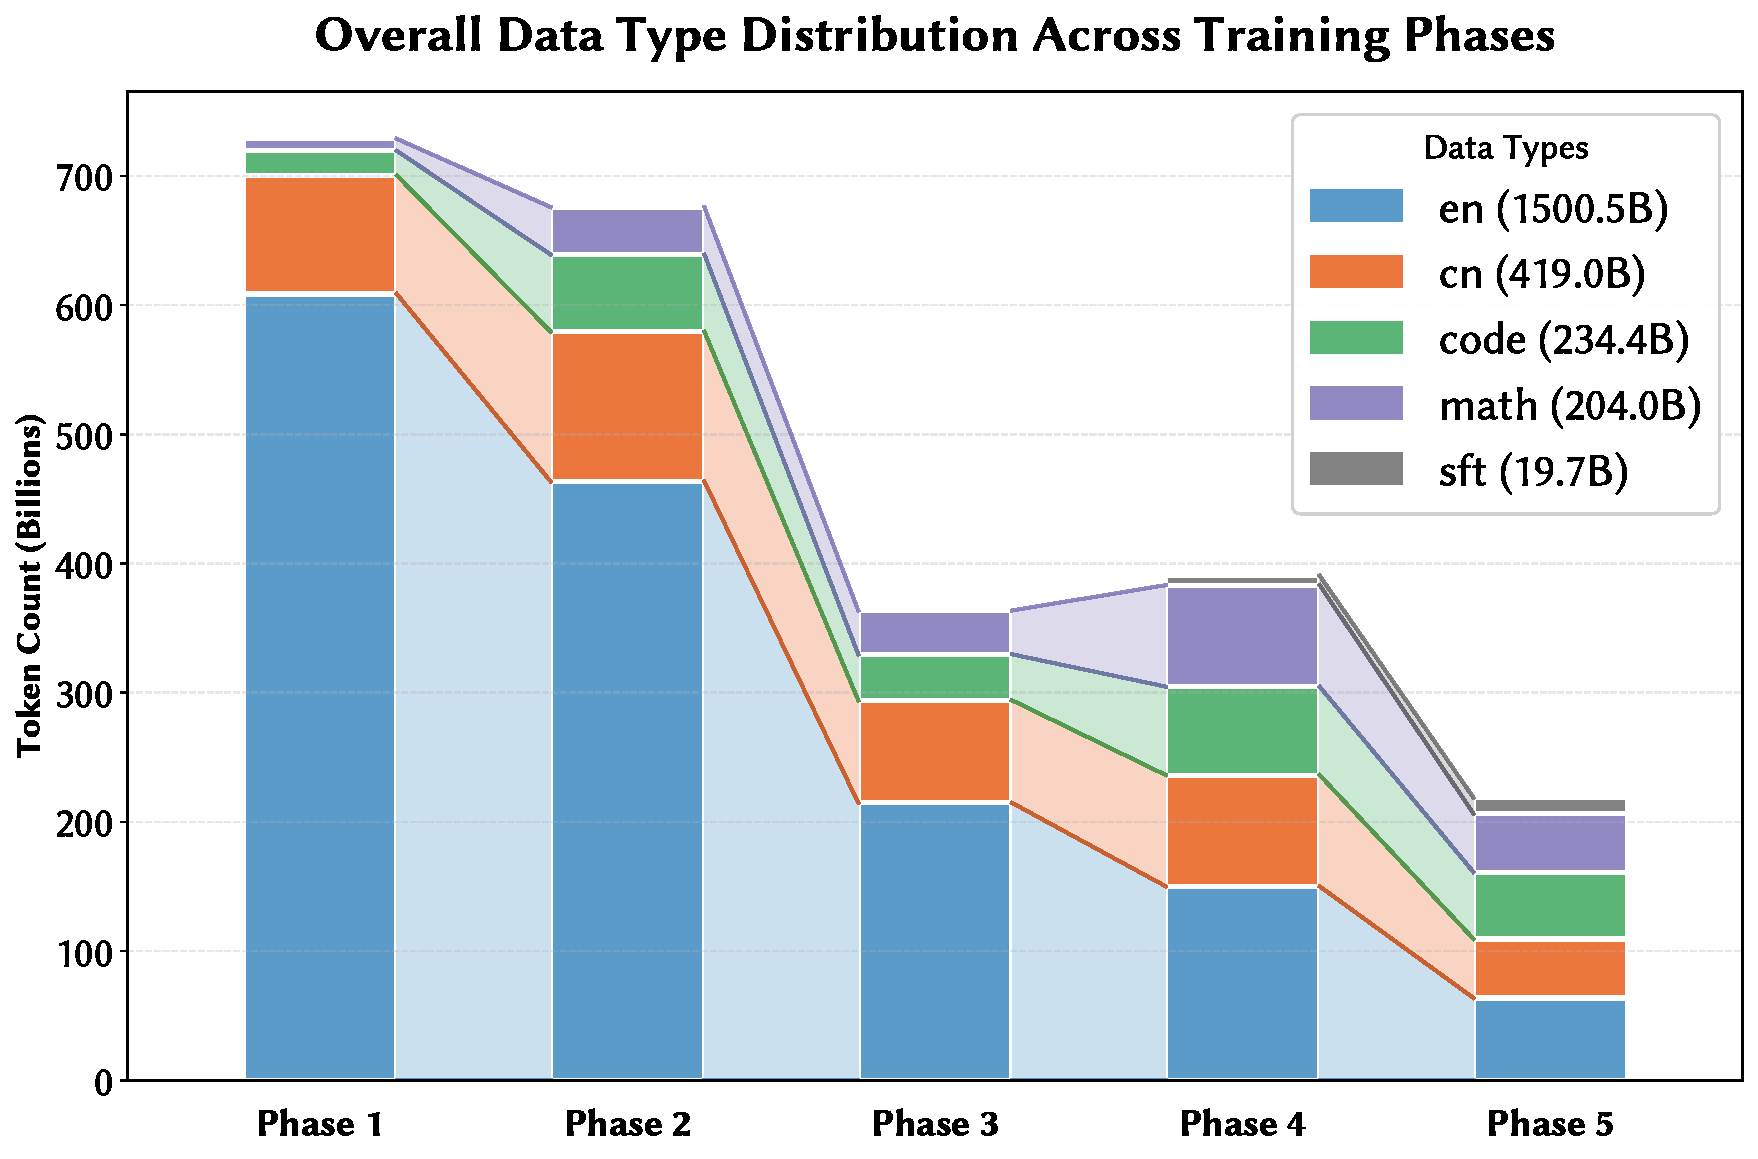
\includegraphics[width=\linewidth]{fig/overall_type_flow.pdf}
        \caption{Phase-wise data mixture transitions}
    \end{subfigure}%
    \hfill
    \begin{subfigure}[b]{0.49\textwidth}
        \centering
        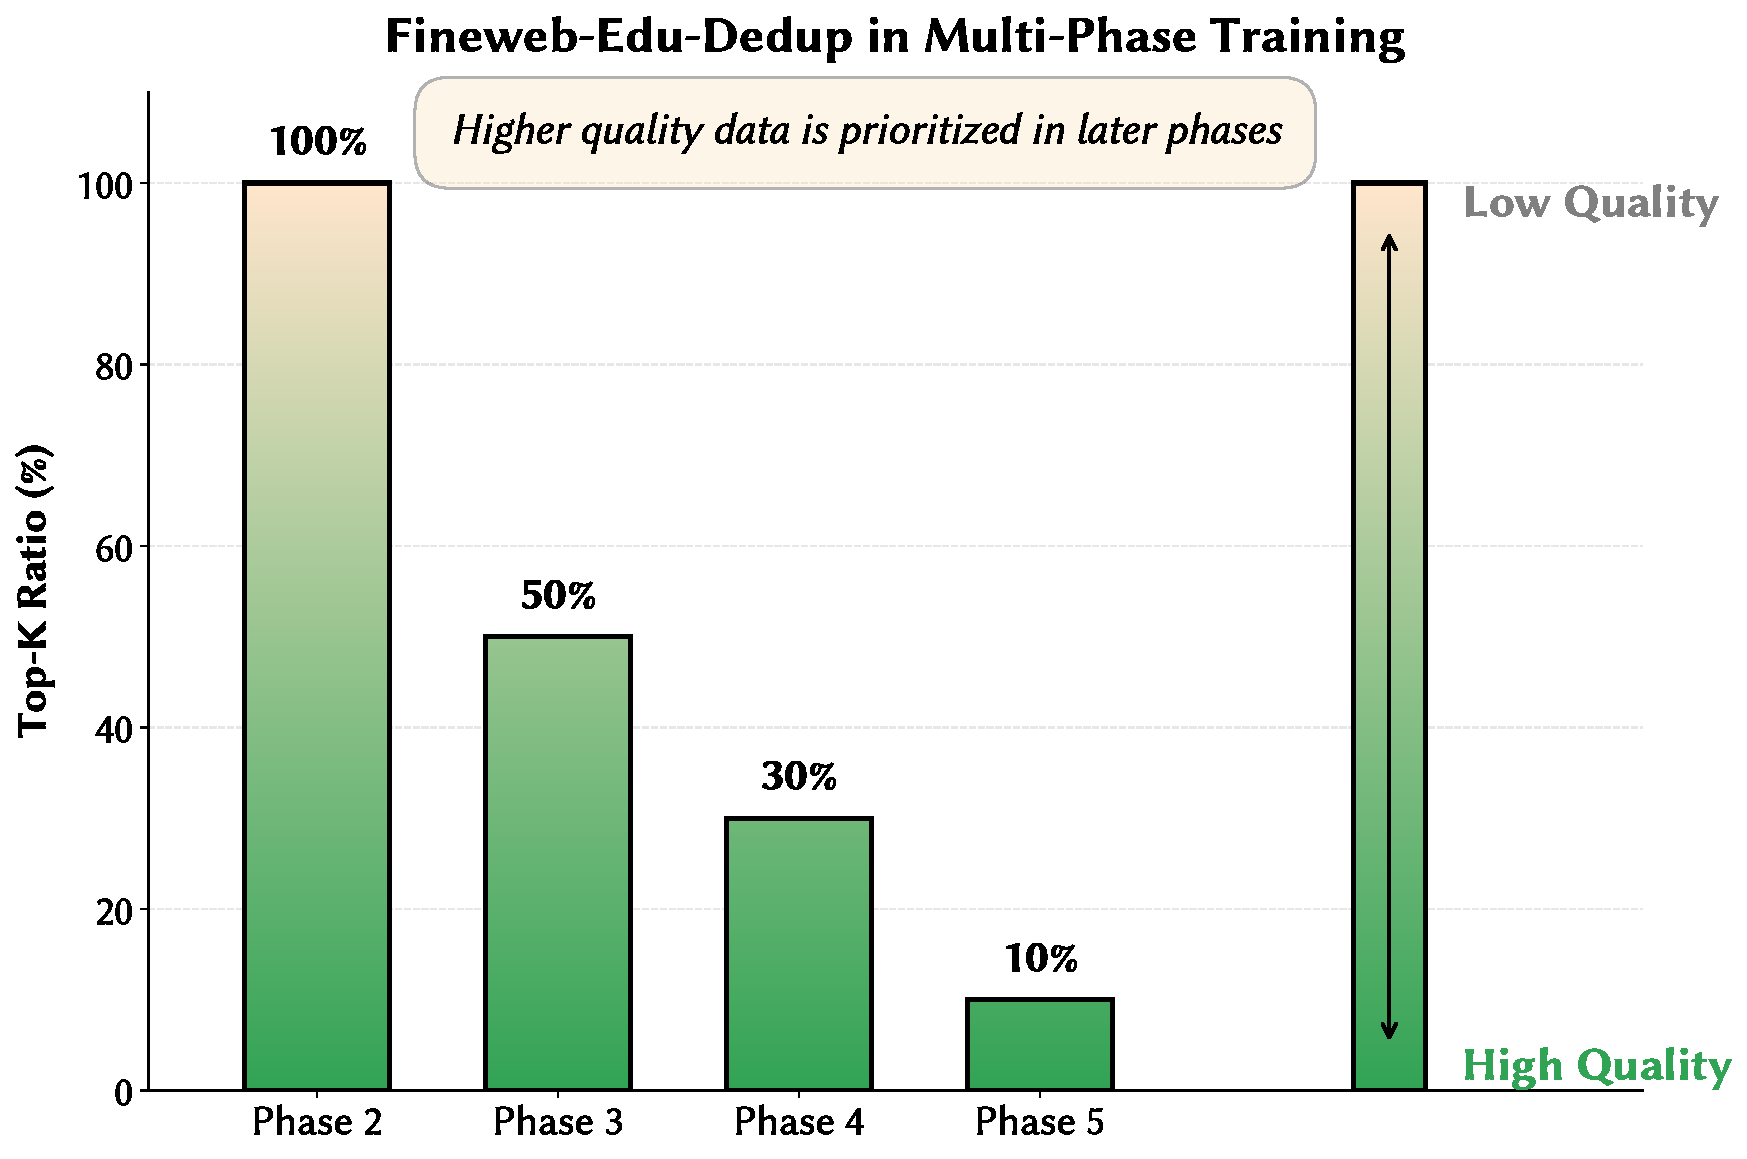
\includegraphics[width=\linewidth]{fig/fineweb_edu_multiphase_gradient.pdf}
        \caption{Phase-wise top-k ratio for Fineweb-Edu}
    \end{subfigure}%
    \caption{Five training phases of \sys. Latter phases keep more refined data samples.}
    \label{fig:data_mixture}
\end{figure}


We structure the training process into five distinct phases with progressive data mixtures, as illustrated in \Cref{fig:data_mixture}. This phased approach incorporates two perspectives of curriculum strategies: domain-level progression and quality-based selection and repetition.

First, we implement a domain-level curriculum by gradually increasing the proportion of Chinese, code, and mathematical datasets in later phases, while introducing supervised fine-tuning data in the final two phases. The phase-wise mixture transitions are visualized in \Cref{fig:data_mixture}. To keep training stability, we maintain English content above 30\% while limiting Chinese, code, and mathematical content each below 30\%. The specific domain mixtures are detailed in \Cref{tab:phase1_stats,tab:phase2_stats,tab:phase3_stats,tab:phase4_stats,tab:phase5_stats}.

Second, we apply quality-based filtering within each domain during later phases, retaining only high-scoring partitions based on available quality metrics. Specifically, one dataset can occur in multiple phases rather than appear only once in the whole training process. However, in each phase, each data sample mostly occurs only once. Moreover, instead of repeating the whole dataset, we mostly keep only the high-quality partition and progressively decrease top-k retention ratios across phases, effectively increasing average data quality, for datasets with a quality metric. 
For example, as shown in \Cref{fig:data_mixture}, we use the entire Fineweb-Edu dataset in phase two, then retain only 50\%, 30\%, and 10\% of top-quality samples in subsequent phases. This selective repetition strategy ensures that the top 10\% samples are exposed to the model four times throughout training, while lower-quality samples appear only once.

This selective repetition serves two primary purposes. On the one hand, we experimentally find that mildly repeating a high-quality portion can attain better training efficiency than one-pass training. We validate this approach using a 1.5B Qwen2.5 model trained on 30B tokens from a DCLM-Baseline shard. As shown in Table~\ref{tab:curriculum_comparison}, retaining 33.4\% of top-quality samples for three epochs outperforms one-pass training, demonstrating the efficacy of strategic repetition. More repetition on the aggressive filtered subset can improve even more on benchmarks like MMLU, but can impede other general capabilities. Experimental details are in \Cref {sec:reference_repetition_curriculum}. A similar experiment is conducted in D4~\citep{tirumala2025d4} while we step forward to explore the effect of filtering and repetition on different capability dimensions, rather than on merely PPL or loss perspective. On the other hand, repetition compensates for aggressive deduplication, as high-quality content naturally occurs more frequently in the internet and can also serve as an indicator of data quality. Prior research indicates that mild multi-epoch training (under four repetitions) preserves sample utility, with larger datasets tolerating more repetition~\citep{yan2025largerdatasetsrepeatedmore,muennighoff2023data_constrained}.

\subsection{Multi-Dataset Data Curriculum}\label{sec:multi_dataset_curriculum_subsec}

Beyond phase-level adjustments, we construct instance-level curriculum learning within each phase. To fully take advantage of the data curriculum, we adopt the technique of Curriculum Model Average (CMA)~\citep{luo2025learningratedecaywastes}, which adopts appropriate learning rate scheduling and model averaging in curriculum-based pretraining. As demonstrated in \Cref{tab:curriculum_comparison}, CMA outperforms uniform sampling in our 1.5B model experiments. We discuss the small-scale reference experiment in \Cref{sec:reference_repetition_curriculum} in detail.

However, the pretraining dataset mostly consists of data samples from various source corpora and constructing a multi-dataset curriculum will present new challenges. Different datasets may employ distinct quality metrics or lack them entirely. To address this, we propose the three-step procedure outlined in \Cref{alg:multi-domain-curriculum} and \Cref{fig:multi_domain_curriculum}:

\begin{enumerate}
    \item \textbf{Within-Dataset Ranking}: Samples within each dataset are independently sorted using dataset-specific quality metrics in ascending order. For datasets without quality labels, we assign random scores uniformly distributed in $[0,1]$ to enable shuffling within the curriculum framework.
    \item \textbf{Rank Rescaling}: Dataset-specific ranks are normalized to a global scale using:
    \[
    R_{\text{global}}(x_A) = r_A \times \frac{N_{\text{total}}}{N_A}
    \]
    where $r_A$ is the within-dataset rank, $N_A$ is the dataset sample count, and $N_{\text{total}}$ is the total sample count.
    
    \item \textbf{Global Interleaving}: All samples are merged and sorted by their rescaled global ranks.
\end{enumerate}

This algorithm ensures: (1) preservation of within-dataset quality ordering or shuffling the dataset without quality labels, (2) proportional interleaving across datasets according to mixture ratios, and (3) maintenance of stable dataset mixtures throughout training. The mixture of datasets is heuristically designed with reference to the quantile benchmarking results in \Cref{sec:data_benchmark}.

\begin{algorithm}[t]
\caption{Multi-Dataset Curriculum Construction}
\label{alg:multi-domain-curriculum}
\begin{algorithmic}[1]
\Require Datasets $D_1, D_2, \dots, D_k$ with their specific quality metrics
\Ensure Multi-dataset curriculum dataset
\State $\displaystyle N_{\text{total}} \gets \sum_{i=1}^k |D_i|$ \Comment{Compute total sample count}
\For{each dataset $D_i$}
    \State (Optionally) Add a random number for the dataset without a quality label
    \State Sort $D_i$ by dataset-specific quality metric (ascending) \Comment{Within-dataset ranking}
    \State Assign ordinal ranks $r_i(x) \in [1, |D_i|]$ to each sample $x \in D_i$
    \State Compute rescaled ranks: $R(x) \gets r_i(x) \times \frac{N_{\text{total}}}{|D_i|}$ for all $x \in D_i$
\EndFor
\State $\displaystyle U \gets \bigcup_{i=1}^k D_i$ \Comment{Combine all datasets}
\State Sort $U$ by rescaled rank $R(x)$ in ascending order \Comment{Global interleaving}
\State \Return sorted $U$
\end{algorithmic}
\end{algorithm}

In practice, we implement this multi-dataset curriculum in the final three training phases to avoid low-quality samples being sorted together and fed to an immature model, which can result in instability. We set the final learning rate to $6\times 10^{-4}$ and average the last six checkpoints, as detailed in Section~\ref{sec:training_configuration}.

\begin{figure}[t!]
    \centering
    
\includegraphics[width=1.0\linewidth]{multi_domain_curriculum_algorithm.pdf}
    \caption{Multi-Dataset Curriculum Construction Process.}
    \label{fig:multi_domain_curriculum}
\end{figure}

\subsection{Pretraining Configuration and Implementation}
\label{sec:training_configuration}

\paragraph{Model Architecture.} Our 2B-parameter model architecture primarily refers to Qwen3-1.7B~\citep{qwen3} with modifications for training stability. We untie word embeddings to reduce communication overhead, resulting in 1.4B non-embedding parameters and 0.6B embedding parameters. To ensure FP16 training stability, we incorporate QK-norm, sandwich norm, and soft capping (detailed in \Cref{sec:architecture_stability}). Complete architectural specifications are provided in \Cref{tab:training_config}.

\paragraph{Training Hyperparameters.} We train with a context length of 4096 and a batch size of 2048. We run small-scale experiments with a 1.5B model on 30B tokens at a batch size of 512, and then extrapolate roughly an optimal peak learning rate of $5\times 10^{-3}$ via square-root scaling~\citep{malladi2022sqrtrule}. We employ a Warmup-Stable-Decay schedule~\citep{hu2024minicpmunveilingpotentialsmall} and reduce the peak learning rate from $5\times 10^{-3}$ to $3\times 10^{-3}$ after the first phase to mitigate the instability caused by data distribution shift effects. The learning rate remains constant through phases 2--4, then decays to $6\times 10^{-4}$ in phase 5 to accommodate the multi-dataset curriculum~\citep{luo2025learningratedecaywastes}. We average the final eight checkpoints (saved every 3.36B tokens) to reduce variance from insufficient learning rate decay, with model averaging details provided in \Cref{sec:model_average}.

\paragraph{Training Curve Analysis.}
\Cref{fig:lr_loss} presents learning rate, training loss, and validation loss trajectories. Two key observations emerge:

\begin{enumerate}
    \item Training loss exhibits non-standard decay patterns due to three factors: (1) the learning rate reductions between phase 1 and phase 2 induce abrupt loss drop at the phase transition, (2) in later phases,  we introduce increased low-perplexity code and mathematical content, which results in continually decreasing loss, and (3) the quality-based curricula import more high-quality data in latter steps within phases 3--5, which accelerates convergence of loss, followed by slight increases at phase transitions.
    
    \item Validation loss on a DCLM-Baseline subset shows similar phase-transition drops but anomalous increases during phases 3--4. These increases likely reflect domain misalignment between the validation set (primarily English text) and training data (increasing code and mathematical content). Each phase ends with accelerated validation loss decay (benefiting from high-quality data) followed by sharp increases (probably from distribution shifts by curriculum).
\end{enumerate}

These patterns suggest that more diverse validation sets would better track training progress. Future work should consider more gradual domain transitions and increased phase counts for improved training stability.


\begin{figure}
    \centering
    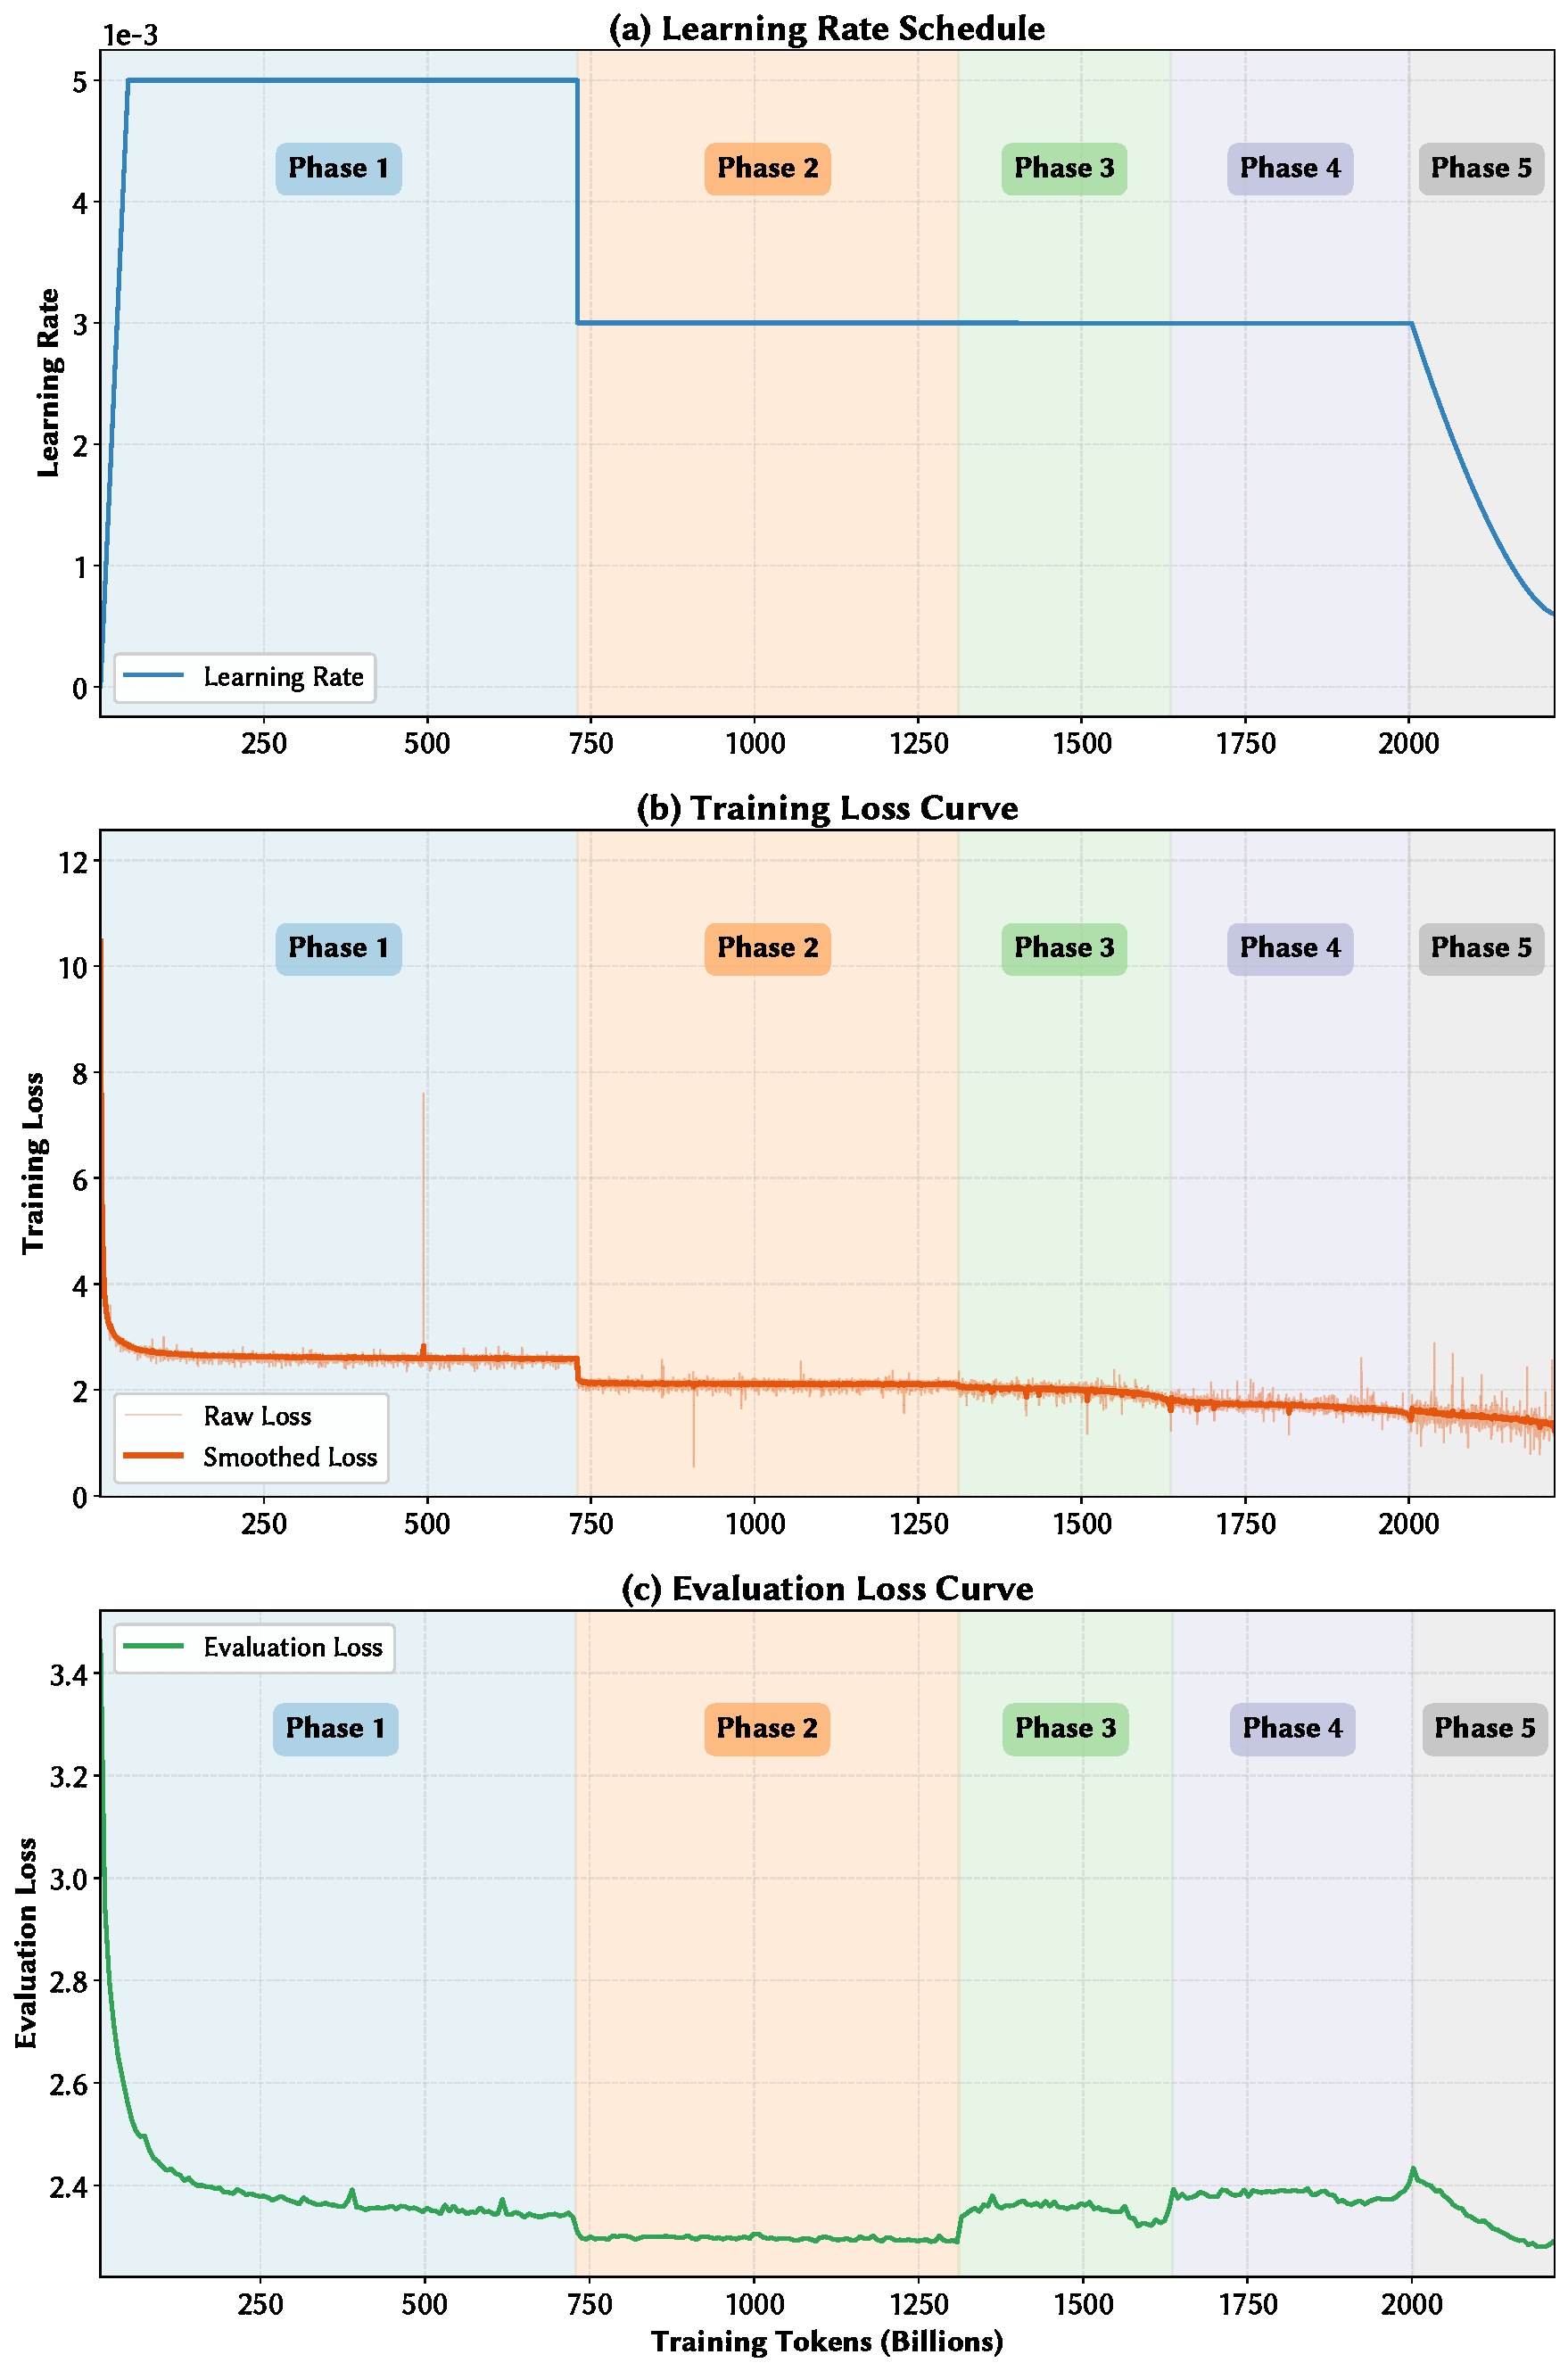
\includegraphics[width=0.9\linewidth]{fig/combined_metrics.pdf}
    \caption{Learning Rate Schedule, Training Loss, and Validation Loss Curves.}
    \label{fig:lr_loss}
\end{figure}












    







    
    


    









